 \documentclass[journal,12pt,twocolumn]{IEEEtran}
\usepackage{amsthm}
\allowbreak
\usepackage{setspace}
\usepackage{gensymb}
\singlespacing
\usepackage[cmex10]{amsmath}
\usepackage{caption}
\usepackage{amsthm}
\usepackage{float}
\DeclareUnicodeCharacter{2212}{-}
\usepackage{tikz}
\usepackage{pgfplots}

\usepackage{mathrsfs}
\usepackage{txfonts}
\usepackage{stfloats}
\usepackage{bm}
\usepackage{cite}
\usepackage{cases}
\usepackage{subfig}

\usepackage{longtable}
\usepackage{multirow}

\usepackage{enumitem}
\usepackage{mathtools}
\usepackage{steinmetz}
\usepackage{tikz}
\usepackage{circuitikz}
\usepackage{verbatim}
\usepackage{tfrupee}
\usepackage[breaklinks=true]{hyperref}
\usepackage{graphicx}
\usepackage{tkz-euclide}
\graphicspath{ {./images/} }
\usetikzlibrary{calc,math}
\usepackage{listings}
    \usepackage{color}                                            %%
    \usepackage{array}                                            %%
    \usepackage{longtable}                                        %%
    \usepackage{calc}                                             %%
    \usepackage{multirow}                                         %%
    \usepackage{hhline}                                           %%
    \usepackage{ifthen}                                           %%
    \usepackage{lscape}     
\usepackage{multicol}
\usepackage{chngcntr}
\usepackage{tikz}
\usetikzlibrary{automata,positioning}

\DeclareMathOperator*{\Res}{Res}

\renewcommand\thesection{\arabic{section}}
\renewcommand\thesubsection{\thesection.\arabic{subsection}}
\renewcommand\thesubsubsection{\thesubsection.\arabic{subsubsection}}

\renewcommand\thesectiondis{\arabic{section}}
\renewcommand\thesubsectiondis{\thesectiondis.\arabic{subsection}}
\renewcommand\thesubsubsectiondis{\thesubsectiondis.\arabic{subsubsection}}
\renewcommand{\figurename}{Fig.}


\hyphenation{op-tical net-works semi-conduc-tor}
\def\inputGnumericTable{}                                 %%

\lstset{
%language=C,
frame=single, 
breaklines=true,
columns=fullflexible
}
\begin{document}


\newtheorem{theorem}{Theorem}[section]
\newtheorem{problem}{Problem}
\newtheorem{proposition}{Proposition}[section]
\newtheorem{lemma}{Lemma}[section]
\newtheorem{corollary}[theorem]{Corollary}
\newtheorem{example}{Example}[section]
\newtheorem{definition}[problem]{Definition}
\newcommand{\comb}[2]{{}^{#1}\mathrm{C}_{#2}}
\newcommand{\BEQA}{\begin{eqnarray}}
\newcommand{\EEQA}{\end{eqnarray}}
\newcommand{\define}{\stackrel{\triangle}{=}}
\bibliographystyle{IEEEtran}
\raggedbottom
\setlength{\parindent}{0pt}
\providecommand{\mbf}{\mathbf}
\providecommand{\pr}[1]{\ensuremath{\Pr\left(#1\right)}}
\providecommand{\qfunc}[1]{\ensuremath{Q\left(#1\right)}}
\providecommand{\sbrak}[1]{\ensuremath{{}\left[#1\right]}}
\providecommand{\lsbrak}[1]{\ensuremath{{}\left[#1\right.}}
\providecommand{\rsbrak}[1]{\ensuremath{{}\left.#1\right]}}
\providecommand{\brak}[1]{\ensuremath{\left(#1\right)}}
\providecommand{\lbrak}[1]{\ensuremath{\left(#1\right.}}
\providecommand{\rbrak}[1]{\ensuremath{\left.#1\right)}}
\providecommand{\cbrak}[1]{\ensuremath{\left\{#1\right\}}}
\providecommand{\lcbrak}[1]{\ensuremath{\left\{#1\right.}}
\providecommand{\rcbrak}[1]{\ensuremath{\left.#1\right\}}}
\theoremstyle{remark}
\newtheorem{rem}{Remark}
\newcommand{\sgn}{\mathop{\mathrm{sgn}}}
\providecommand{\abs}[1]{$\left\vert#1\right\vert$}
\providecommand{\res}[1]{\Res\displaylimits_{#1}} 
\providecommand{\norm}[1]{$\left\lVert#1\right\rVert$}
%\providecommand{\norm}[1]{\lVert#1\rVert}
\providecommand{\mtx}[1]{\mathbf{#1}}
\providecommand{\mean}[1]{E$\left[ #1 \right]$}
\providecommand{\fourier}{\overset{\mathcal{F}}{ \rightleftharpoons}}
%\providecommand{\hilbert}{\overset{\mathcal{H}}{ \rightleftharpoons}}
\providecommand{\system}{\overset{\mathcal{H}}{ \longleftrightarrow}}
	%\newcommand{\solution}[2]{\textbf{Solution:}{#1}}
\newcommand{\solution}{\noindent \textbf{Solution: }}
\newcommand{\cosec}{\,\text{cosec}\,}
\providecommand{\dec}[2]{\ensuremath{\overset{#1}{\underset{#2}{\gtrless}}}}
\newcommand{\myvec}[1]{\ensuremath{\begin{pmatrix}#1\end{pmatrix}}}
\newcommand{\mydet}[1]{\ensuremath{\begin{vmatrix}#1\end{vmatrix}}}
\numberwithin{equation}{subsection}
\makeatletter
\@addtoreset{figure}{problem}
\makeatother
\let\StandardTheFigure\thefigure
\let\vec\mathbf
\renewcommand{\thefigure}{\theproblem}
\def\putbox#1#2#3{\makebox[0in][l]{\makebox[#1][l]{}\raisebox{\baselineskip}[0in][0in]{\raisebox{#2}[0in][0in]{#3}}}}
     \def\rightbox#1{\makebox[0in][r]{#1}}
     \def\centbox#1{\makebox[0in]{#1}}
     \def\topbox#1{\raisebox{-\baselineskip}[0in][0in]{#1}}
     \def\midbox#1{\raisebox{-0.5\baselineskip}[0in][0in]{#1}}
\vspace{3cm}
\title{AI1103: Assignment 5}
\author{Damaragidda Bharadwaja Rao - CS20BTECH11012}
\maketitle
\newpage
\bigskip
\renewcommand{\thefigure}{\theenumi}
\renewcommand{\thetable}{\theenumi}
Download all latex-tikz codes from 
\begin{lstlisting}
https://github.com/Bharadwaja-rao-D/AI1103/blob/main/assignment5/assignment5.tex
\end{lstlisting}
\section*{Problem UGC-MATH 2019 Q 105:}
Consider a simple symmetric random walk on integers, where from every state i you move to i-1 and i+1 with the probability half each. Then which of the following are true?
\begin{enumerate}
\item The random walk is aperiodic
\item The random walk is irreducible
\item The random walk is null recurrent 
\item The random walk is positive recurrent
\end{enumerate}
\section*{Solution:}
The simple symmetric random walk is a Markov chain with state space S = $\{i | i \in \mathbb{Z}\}$ and with transition matrix P where, 
\begin{equation}
 p_{ij} =\begin{cases}
  0 , &|i-j|>1\vspace{0.2cm}\\
  p = \dfrac{1}{2} , &j = i+1\vspace{0.2cm}\\
  q =1-p = \dfrac{1}{2} , &j = i-1\\
  \end{cases}
\end{equation}
and $p_{ij}$ denotes the probability of being in state j, starting from state i after n steps or transitions.
\renewcommand{\thefigure}{1}
\begin{figure}[h]
	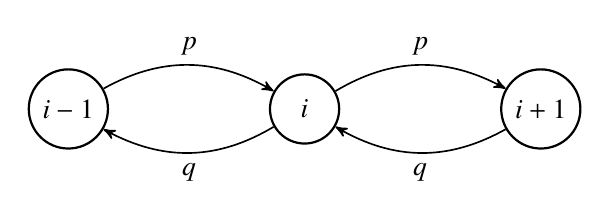
\begin{tikzpicture}[->, >=stealth', auto, semithick, node distance=3cm]
	\tikzstyle{every state}=[fill=white,draw=black,thick,text=black,scale=1]
	\node[state]    (A)                     {$i-1$};
	\node[state]    (B)[right of=A]   {$i$};
	\node[state]    (C)[right of=B]   {$i+1$};
	\path
	(A) edge[bend left,above]			node{$p$}	(B)
	(B) edge[bend left,below]	node{$q$}	(A)
	edge[bend left,above]		node{$p$}	(C)
	(C) edge[bend left,below]	node{$q$}	(B);
	\end{tikzpicture}
	\caption{Simple Symmetric random walk on integers}
\end{figure}
\renewcommand{\thefigure}{2}
\begin{figure}[H]
\begin{align}
P = \bordermatrix{& \ldots & -2&-1&0&1&2&\ldots \cr
                \vdots & \vdots & \vdots & \vdots & \vdots & \vdots & \vdots & 						\vdots\cr
                -2& \ldots & 0  & p & 0 & 0 & 0 &\ldots\cr
                -1& \ldots & q  & 0 & p & 0 & 0 &\ldots\cr
                 0& \ldots & 0  & q & 0 & p & 0 &\ldots\cr
				 1& \ldots & 0  & 0 & q & 0 & p &\ldots\cr
				 2& \ldots & 0  & 0 & 0 & q & 0 &\ldots\cr	                
                \vdots & \vdots & \vdots & \vdots & \vdots & \vdots & \vdots & 						\vdots\cr
                }
\end{align}
\caption{Transition matrix of the Markov chain }
\end{figure}
\begin{enumerate}
\item For a Markov chain to be aperiodic there should exist an integer k such that
\begin{align}
p^n_{jj} > 0 \hspace{0.5cm} \forall n \geq k \label{eq:aperoidic}
\end{align} 
to return to same state after n steps, number of forward and backward steps should be same, that is number of steps should be even. 
\begin{align}
p^n_{jj} = 0 \hspace{0.5cm} \forall n \in Odd \label{eq:1}
\end{align}
$\therefore$ Equation \eqref{eq:aperoidic} is not satisfied and Option \textbf{(1)} is \textbf{incorrect}.
\item For a Markov chain to be \textbf{irreducible} all pairs i,j should communicate with each other.Let us assume that the chain starts from state i and let us assume that it requires m forward and (n-m) backward steps to reach j .Let $i < j$ wlog 
\begin{align}
j - i &= m - (n - m) = 2m - n\\
m &= \frac{(j - i) + n}{2}\\
p_{ij} &= \comb{n}{m} p^m q^{n-m}
\end{align}
\begin{multline}
p_{ij} = \comb{n}{\brak{\dfrac{(j - i) + n}{2}}} p^m q^{n-m} > 0\\
 n = (j-i)+2k \hspace{0.2cm} \forall k \in \mathbb{W}
\end{multline}
Here i and j are general , hence all pairs i and j communicate with each other.\\
$\therefore$Option \textbf{(2)} is \textbf{correct}
\item In a Markov Chain for state i to be \textbf{recurrent} it should satisfy ,
\begin{align}
\lim_{t \to \infty} \sum_{n=1}^{t} p^n_{ii} = \infty \label{eq:Recurrent}
\end{align}
\begin{align}
\lim_{t \to \infty} \sum_{n=1}^{t} p^n_{ii} &= \lim_{t \to \infty}\left(\sum_{k=1}^{t} p^{2k}_{ii} + \sum_{k=1}^{t} p^{(2k-1)}_{ii}\right)\\
&= \lim_{t \to \infty}\sum_{k=1}^{t} p^{2k}_{ii}\\
p^{2k}_{ii} &= \comb{2k}{k}p^kq^k  = \frac{2k !}{k!k!}p^kq^k \label{eq:2}
\end{align}
By using Stirling approximation to the \eqref{eq:2} we get 
\begin{align}
&p^{2k}_{ii} = \dfrac{ \left((2k)^{2k+\frac{1}{2}}\right)\times \exp(-2k)\times(2\pi)^{\frac{1}{2}}}{\left(k^{k+\frac{1}{2}}\times \exp(-k)\right)^2\times
2\pi}p^kq^k\\
&= \dfrac{(4pq)^{2k}}{(k\pi)^{\frac{1}{2}}} = \dfrac{1}{(k\pi)^{\frac{1}{2}}}\\
&\lim_{t \to \infty}\sum_{k=1}^{t} p^{2k}_{ii} = \lim_{t \to \infty}\sum_{k=1}^{t} \dfrac{1}{(k\pi)^{\frac{1}{2}}}
\end{align}
Since $\dfrac{1}{k^\frac{1}{2}}$ is divergent, Equation \eqref{eq:Recurrent} is satisfied\\
$\therefore$ The random walk is \textbf{recurrent}\\
The first-passage time probability is 
\begin{multline}
f_{i,j}(n) = \Pr(X_n = j, X_{n-1} \neq j, X_{n-2} \neq j, ...\\
 X_1 \neq j | X_0 = i )
\end{multline}
The first-passage time $T_{i,j}$ from state i to j has the PMf $f_{i,j}(n)$ and the distribution function
\begin{align}
F_{i,j}(n) = \sum _{k=0}^n f_{i,j}(k) \label{eq:3}
\end{align}
For the Markov Chain to be null recurrent 
\begin{align}
\overline{T_{j,j}} = \infty \label{eq:null recurrent}
\end{align}
and for positive recurrent 
where $\overline{T_{j,j}}$ represents the mean time to enter j starting from j. We can calculate the mean by using the distribution function 
\begin{align}
\overline{T_{j,j}} = 1 + \sum _{k=0}^n \left(1 - F_{j,j}(k)\right) \label{eq:4}
\end{align}
From \eqref{eq:3} and \eqref{eq:4} we get \eqref{eq:null recurrent} condition to be satisfied \\
$\therefore$ Option \textbf{(3)} is \textbf{correct}.
\item For a Markov chain to be positive recurrent it should satisfy the following condition
\begin{align}
\overline{T_{j,j}} < \infty \label{eq:positive recurrent}
\end{align}
Since the Markov chain satisfies the \eqref{eq:null recurrent} but not \eqref{eq:positive recurrent} it is not positive recurrent.\\
$\therefore$ Option \textbf{(4)} is \textbf{incorrect}\\
\textbf{Answer :} option2, option3
\end{enumerate}

\end{document}
